\documentclass{beamer}

\usepackage{menukeys}
\usepackage{minted}
\usepackage{svg}

\usetheme{Boadilla}

% Title
\title{Vim Lab}
\author{Ethan Wong}
\date{October 13, 2023}
\institute{Linux Users Group @ UIC}

\begin{document}
\begin{frame}
	\titlepage
\end{frame}

\begin{frame}{Table of Contents}
	\tableofcontents[pausesections]
\end{frame}

\section{Why Vim?}
\begin{frame}{Why Vim?}
	\begin{itemize}
		\item Simple and ubiquitous text editor 
		\item Usable in a \textit{terminal}
		\item Keyboard-centric, meaning that a mouse is
			\underline{optional}
		\item Vim's version of modal input is popular and commonly emulated
		\item Part of the POSIX standard!
	\end{itemize}
\end{frame}

\section{History}
\begin{frame}{Table of Contents}
	\tableofcontents[currentsection]
\end{frame}

\begin{frame}{History}
	\begin{columns}
		\begin{column}{0.5\textwidth}
			\begin{itemize}
				\item Vi(no -m) was created by Bill Joy in \textbf{1976} for the
					Second BSD.\footnotemark
					\pause

				\item It is the visual mode for the \texttt{ex}
					command line text editor.
					\pause

				\item Vi was created for remote editing over a \textit{300} baud
					modem, which transmitted text slower than you can read!
					\pause
			\end{itemize}
		\end{column}
		\begin{column}{0.5\textwidth}
			\begin{figure}
				\centering
				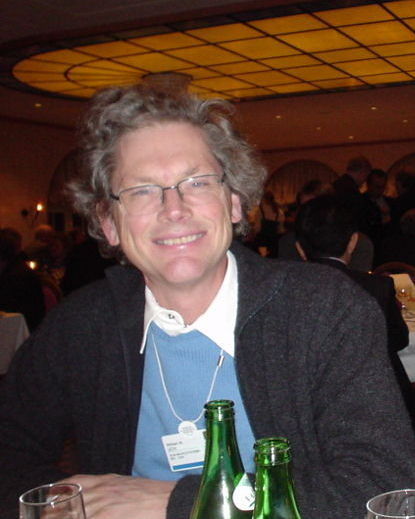
\includegraphics[width=0.5\textwidth]{bill_joy.jpg}
				\caption{Bill Joy, the creator of \texttt{vi}}
			\end{figure}
		\end{column}
	\end{columns}

	\footnotetext{\url{https://web.archive.org/web/20060701083055/http://web.cecs.pdx.edu/~kirkenda/joy84.html}}
\end{frame}

\begin{frame}{History}
	\begin{itemize}
		\item Vi iMproved (\texttt{vim}) was created by Bram Moolenaar
			in 1988 as a \textit{clone} of \texttt{vi}.
			\pause

		\item \texttt{vim} is a superset of \texttt{vi}, introducing new
			features such as syntax highlighting, undo/redo, screen
			splitting, and plugin support.
			\pause

		\item Like \texttt{vi}, \texttt{vim} has also been ported to a
			wide range of OS's.
			\pause

		\item Today, \texttt{vim} and its derivatives make up one of the
			most most popular text editor families.\footnotemark
	\end{itemize}

	\footnotetext{\url{https://survey.stackoverflow.co/2023/\#section-most-popular-technologies-integrated-development-environment}}
\end{frame}


\section{Basic Knowledge}
\begin{frame}{Table of Contents}
	\tableofcontents[currentsection]
\end{frame}

\subsection{Goals}
\begin{frame}{Goals}
	We will try to learn:\\
	\begin{itemize}
		\item How to switch between the different \textit{modes}
			of \texttt{vim}
			\pause

		\item How to navigate around a text document using
			\textbf{modal} keybindings
			\pause

		\item Methods for remembering the the mnemonics
			\pause

		\item How to select, manipulate, and insert text into files
			\pause

		\item How to quit \texttt{vim} without restarting your
			computer...\footnote{a.k.a. commands}

	\end{itemize}
\end{frame}

\subsection{Modes}
\begin{frame}{Modes}
	\texttt{vim} is known for a \textbf{modal} editing scheme.
	\pause

	What is modal editing?
	\pause

	In \texttt{vim}, various things that you typically do while editing text
	is split into different \textit{modes}.
	\pause

	\smallskip

	\begin{adjustbox}{max width=\textwidth}
		\begin{tabular}{ | l | l | l | }
			\hline
			\textbf{Mode} & \textbf{Purpose} & \textbf{How to Enter}\\
			\hline
			Normal & Move around and manipulate
			\textit{existing} text & Default, can return to
			by pressing \keys{\escwin} in other modes\\
			\hline
			Insert & Allows you to type text like in any standard
			editor & \keys{i}, \keys{a}, \keys{x}, \keys{c},
			\keys{o}, among others in Normal mode\\
			\hline
			Visual & Allows you to select regions of text as if you
			were using a mouse & \keys{v}, \keys{\shift + v},
			\keys{\ctrl + v} in Normal mode\\
			\hline
			Command & Allows you to execute commands like save and
			exit & \keys{:} in Normal mode\\
			\hline
		\end{tabular}
	\end{adjustbox}
	\smallskip
	\pause

	There are other additional modes that \texttt{vim} has out-of-the-box,
	but these are the basics.
	\pause

	Why should editing be split into modes?
\end{frame}

\subsection{Keybinds}
\begin{frame}{Keybinds}
	Modes allow for \texttt{vim} perform actions using simple and easy to
	remember keystroke sequences! \pause These are known as motions!
	\pause

	\begin{exampleblock}{Example}
		Navigating can be done with \keys{h}, \keys{j}, \keys{k},
		\keys{l} in Normal mode. These corrispond to \keys{\arrowkeyleft},
		\keys{\arrowkeydown}, \keys{\arrowkeyup}, \keys{\arrowkeyright}
		respectively.\footnote{People consider using the arrow keys in
		\texttt{vim} a cardinal sin.}
		\pause

		This allows you to keep your hands on the home-row of your
		keyboard (especially good if you are a touch-typist)!
	\end{exampleblock}
	\pause

	\begin{exampleblock}{Example 2}
		Additionally, an arbitrary number can be prefixed to
		\underline{modify} motions.
		\pause

		One usecase is \keys{5 + j}, which moves down 5 lines in one
		input sequence.
	\end{exampleblock}
\end{frame}

\begin{frame}{Keybinds}
	How can you easily remember these keybinds?
	\pause

	Most keybinds are \textbf{mnemonics} for their corrisponding action.
	\begin{itemize}
		\item \keys{i}nsert enters Insert mode
		\item \keys{a}ppend is the same as insert, but starts
			inserting at the character after the cursor
		\item \keys{x}-out deletes a single character
		\item \keys{d}elete takes your selection and deletes it
		\item \keys{c}hange deletes your selection and enters Insert
			mode
		\item etc.
	\end{itemize}
	\pause

	There are a billion keybinds in \texttt{vim}, so don't fret about
	learning all of them at once. Learning as you go is the method here!
\end{frame}

\begin{frame}[fragile]{Keybinds}
	\texttt{vim} motions are extremely powerful. They let you condense the
	work of selecting text and changing it into easy to remember input
	sequences!
	\pause

	\begin{exampleblock}{Example 1}
		\keys{cc} lets you delete a line and start retyping text in one
		shot (\keys{c}hange a line)! Double pressing most actions will
		allow you to apply it to the line your cursor is on.
		\pause

		\bigskip

		\begin{columns}
			\begin{column}{0.5\textwidth}
				\textbf{Before}
				\begin{verbatim}
				This is a sentence!
				The cursor is below this line.
				_Emacs users are stinky :(
				another wacky line!
				\end{verbatim}
			\end{column}
			\begin{column}{0.5\textwidth}
				\textbf{After}
				\begin{verbatim}
				This is a sentence!
				The cursor is below this line.
				|
				another wacky line!
				\end{verbatim}
			\end{column}
		\end{columns}
	\end{exampleblock}
\end{frame}

\begin{frame}[fragile]{Keybinds}
	\begin{exampleblock}{Example 2}
		\keys{dw} Lets you \keys{d}elete a \keys{w}ord.
		\pause

		The \keys{w} works to specify your selection after
		\underline{any} action! So, this will work with \keys{c} too!
		\pause

		\medskip

		\begin{columns}
			\begin{column}{0.5\textwidth}
				\textbf{Before}
				\begin{verbatim}
				This is a sentence!
				The cursor is below this line.
				_Emacs users are stinky :(
				another wacky line!
				\end{verbatim}
			\end{column}
			\begin{column}{0.5\textwidth}
				\textbf{After}
				\begin{verbatim}
				This is a sentence!
				The cursor is below this line.
				_users are stinky :(
				another wacky line!
				\end{verbatim}
			\end{column}
		\end{columns}
	\end{exampleblock}
\end{frame}

\begin{frame}[fragile]{Keybinds}
	\begin{exampleblock}{Example 3}
		Commands can be chained too!
		\keys{2k} and \keys{dip} Lets you move \keys{2} up (\keys{k})
		and \keys{d}elete the \keys{i}nner
		\keys{p}aragraph.\footnotemark
		\pause

		\bigskip

		\begin{columns}
			\begin{column}{0.5\textwidth}
				\textbf{Before}
				\begin{verbatim}
				This is a sentence!
				The cursor is below this line.
				_Emacs users are stinky :(
				another wacky line!
				\end{verbatim}
			\end{column}
			\begin{column}{0.5\textwidth}
				\textbf{After}
				\begin{verbatim}
				_



				\end{verbatim}
			\end{column}
		\end{columns}
	\end{exampleblock}

	\footnotetext{inner meaning excluding any spacing surrounding the paragraph}
\end{frame}

\begin{frame}{Keybinds}
	Other useful actions include (but not all)...
	\pause

	\begin{itemize}
		\item \keys{o} and \keys{O} which creates a new line below/above
			the current line respectively

		\item \keys{gg} and \keys{G} which puts the cursor at the
			top/bottom of the file

		\item \keys{zz} which centers the editing window

		\item \keys{b} and \keys{e} goes to the \keys{b}eginning and
			\keys{e}nd of the word your cursor is currently on.

		\item \keys{y} to copy (\keys{d} cuts) and \keys{p} to paste

		\item \keys{u} and \keys{\ctrl + r} to undo and redo.
		\item \keys{$\langle\langle$} and \keys{$\rangle\rangle$} to change indentation levels in
			code.
	\end{itemize}
\end{frame}

\subsection{Commands}
\begin{frame}{Table of Contents}
	\tableofcontents[currentsubsection]
\end{frame}

\begin{frame}{Commands}
	There are lots of commands in \texttt{vim}, just like actions, but we'll
	just go over a few. To enter Command mode, just prepend a \keys{:}
	before typing it!
	\pause

	\begin{itemize}
		\item \texttt{:write} or \texttt{:w} saves your
			file\footnote{you can specify a filename afterwards to
			emulate \menu{File>Save As}}
			\pause

		\item \texttt{:quit} or \texttt{:q} quits Vim\footnote{add an
			\texttt{!} to quit and ignore unsaved changes}
			\pause

		\item \texttt{:\%s/<regex>/<regex>/gc} lets you find and replace
			\pause

		\item \texttt{:help <command>} brings up the help-page for any
			Vim command
	\end{itemize}
	\pause

	You can also chain commands, so \texttt{:wq} for example saves your file
	and exits in one shot.\\

	Also, \keys{\textbackslash} and \keys{?} let you search within your
	document.\footnote{use \texttt{:noh} to clear highlighted results after}
	\keys{n} and \keys{N} let you go backwards/forwards through your search
	results.
\end{frame}

\section{Crash Course}
\begin{frame}{Table of Contents}
	\tableofcontents[currentsection]
\end{frame}

\begin{frame}
	Lets try a hands-on demo!
	\pause

	Firstly, open a terminal!
	\begin{itemize}
		\item Windows\\
			Open one of the following:
			\begin{itemize}
				\item Powershell
				\item PuTTy
			\end{itemize}
			You'll need to \texttt{ssh} into
			\texttt{malware.cs.uic.edu}.\\
			Syntax: \texttt{ssh userXX@malware.cs.uic.edu}, where
			$XX$ is a number between 1-25.
		\item MacOS\\
			Simply go to \menu{Applications>Utilities>Terminal} and
			type \texttt{vim}, its included by default!
		\item Linux\\
			Open your terminal of choice, install \texttt{vim} if
			you need to (tho it should be included by default...),
			and run \texttt{vim}.
	\end{itemize}
\end{frame}

\begin{frame}[fragile]{Crash Course}
	\textbf{Challenge!}\\
	I want you to create a simple C program using \texttt{vim} and
	sucessfully compile it! It can be as simple as "Hello, World!" if you'd
	like!

	\begin{minted}{c}
		#include <stdio.h>

		int main(int argc, char **argv) {
			printf("Hello World!\n");
		}
	\end{minted}

	If thats too easy for you, try these extra challenges:
	\begin{itemize}
		\item Don't use the arrow keys at all
		\item Write your program in Rust instead
		\item Do not leave \texttt{vim} at any point when writing the
			program
	\end{itemize}
\end{frame}

\begin{frame}{Crash Course}
	\textbf{Closing Remarks}
	\begin{itemize}
		\item This was a very surface-level introduction to
			\texttt{vim}.\\
			Some features not covered include:
			\begin{itemize}
				\item Vim Modelines
				\item Multiplexing buffers
				\item Macros
				\item Plugins
			\end{itemize}
		\item Don't fret if this is alot of information at once! It's
			important to start small and \underline{learn what you
			need as you go}.
		\item If you want to practice more with \texttt{vim}, try out
			\texttt{vimtutor} which is a guided tutorial to learn
			Vim.
		\item Don't be afraid to reference a cheatsheet like
			\url{https://vim.rtorr.com/} when learning!
		\item As always, practice makes perfect.
	\end{itemize}
\end{frame}

\begin{frame}{Crash Course}
	\begin{center}
		\Huge Thank you!
	\end{center}
\end{frame}

\begin{frame}{Crash Course}
	\begin{columns}
		\begin{column}{0.5\textwidth}
			\textbf{Me :3}
			\begin{figure}
				\centering
				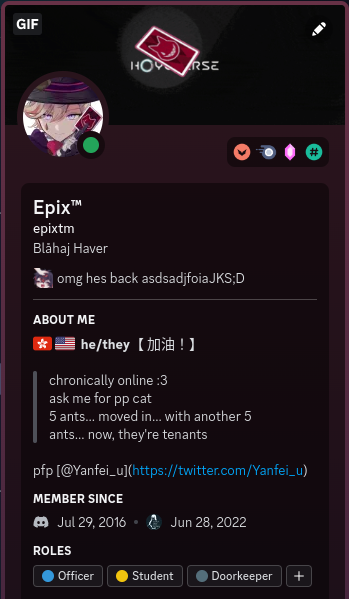
\includegraphics[width=0.60\textwidth]{epixtm.png}
			\end{figure}
		\end{column}
		\begin{column}{0.5\textwidth}
			The information in this presentation will be made
			available\footnotemark on our website!\\
			\url{https://lug.cs.uic.edu}
			
			\bigskip
			Join our Discord!

			\begin{figure}
				\centering
				\includesvg[width=0.5\textwidth]{lug-discord.svg}
				\caption{\url{https://discord.gg/NgxTR7PX5e}}
			\end{figure}
		\end{column}
	\end{columns}

	\footnotetext{sooner or later}
\end{frame}

\end{document}

% vim: set tw=80 ts=4 sw=4:
